\documentclass[a4paper, 12pt]{article}
\usepackage[spanish]{babel}
\usepackage[utf8]{inputenc}
\usepackage{amsmath}
\usepackage{indentfirst}
\usepackage{graphicx}
\usepackage[colorinlistoftodos]{todonotes}
\usepackage{esint}
\usepackage{multicol}
\usepackage{listings}
\usepackage{xcolor}

\usepackage[a4paper,
            bindingoffset=0.2in,
            left=2.5cm,
            right=2.5cm,
            top=2.5cm,
            bottom=2.5cm,
            footskip=30pt]{geometry}

\definecolor{codegreen}{rgb}{0,0.6,0}
\definecolor{codegray}{rgb}{0.5,0.5,0.5}
\definecolor{codepurple}{rgb}{0.58,0,0.82}
\definecolor{backcolour}{rgb}{0.95,0.95,0.92}

\lstdefinestyle{customc}{
	language=C,
    backgroundcolor=\color{backcolour},   
    commentstyle=\color{codegreen},
    keywordstyle=\color{magenta},
    numberstyle=\tiny\color{codegray},
    stringstyle=\color{codepurple},
    basicstyle=\ttfamily\footnotesize,
    breakatwhitespace=false,         
    breaklines=true,                 
    captionpos=b,                    
    keepspaces=true,                 
    numbers=left,                    
    numbersep=5pt,                  
    showspaces=false,                
    showstringspaces=false,
    showtabs=false,                  
    tabsize=2
}

\lstdefinestyle{customasm}{
	language=[x86masm]Assembler,
    backgroundcolor=\color{backcolour},   
    commentstyle=\color{codegreen},
    keywordstyle=\color{magenta},
    numberstyle=\tiny\color{codegray},
    stringstyle=\color{codepurple},
    basicstyle=\ttfamily\footnotesize,
    breakatwhitespace=false,         
    breaklines=true,                 
    captionpos=b,                    
    keepspaces=true,                 
    numbers=left,                    
    numbersep=5pt,                  
    showspaces=false,                
    showstringspaces=false,
    showtabs=false,                  
    tabsize=2
}

\lstset{escapechar=@,style=customasm}

\lstset{literate=
  {á}{{\'a}}1 {é}{{\'e}}1 {í}{{\'i}}1 {ó}{{\'o}}1 {ú}{{\'u}}1
  {Á}{{\'A}}1 {É}{{\'E}}1 {Í}{{\'I}}1 {Ó}{{\'O}}1 {Ú}{{\'U}}1
  {à}{{\`a}}1 {è}{{\`e}}1 {ì}{{\`i}}1 {ò}{{\`o}}1 {ù}{{\`u}}1
  {À}{{\`A}}1 {È}{{\'E}}1 {Ì}{{\`I}}1 {Ò}{{\`O}}1 {Ù}{{\`U}}1
  {ä}{{\"a}}1 {ë}{{\"e}}1 {ï}{{\"i}}1 {ö}{{\"o}}1 {ü}{{\"u}}1
  {Ä}{{\"A}}1 {Ë}{{\"E}}1 {Ï}{{\"I}}1 {Ö}{{\"O}}1 {Ü}{{\"U}}1
  {â}{{\^a}}1 {ê}{{\^e}}1 {î}{{\^i}}1 {ô}{{\^o}}1 {û}{{\^u}}1
  {Â}{{\^A}}1 {Ê}{{\^E}}1 {Î}{{\^I}}1 {Ô}{{\^O}}1 {Û}{{\^U}}1
  {ã}{{\~a}}1 {ẽ}{{\~e}}1 {ĩ}{{\~i}}1 {õ}{{\~o}}1 {ũ}{{\~u}}1
  {Ã}{{\~A}}1 {Ẽ}{{\~E}}1 {Ĩ}{{\~I}}1 {Õ}{{\~O}}1 {Ũ}{{\~U}}1
  {œ}{{\oe}}1 {Œ}{{\OE}}1 {æ}{{\ae}}1 {Æ}{{\AE}}1 {ß}{{\ss}}1
  {ű}{{\H{u}}}1 {Ű}{{\H{U}}}1 {ő}{{\H{o}}}1 {Ő}{{\H{O}}}1
  {ç}{{\c c}}1 {Ç}{{\c C}}1 {ø}{{\o}}1 {å}{{\r a}}1 {Å}{{\r A}}1
  {€}{{\euro}}1 {£}{{\pounds}}1 {«}{{\guillemotleft}}1
  {»}{{\guillemotright}}1 {ñ}{{\~n}}1 {Ñ}{{\~N}}1 {¿}{{?`}}1 {¡}{{!`}}1  {°}{{$^\circ$}}1
}

\setlength{\marginparwidth}{2cm}
\begin{document}
\begin{titlepage}
	\begin{center}
		{\large{UNIVERSIDAD TECNOLÓGICA NACIONAL}}
	\end{center}
	\vspace{15pt}
	\begin{figure}[!ht]
		\centering
		\begin{center}
			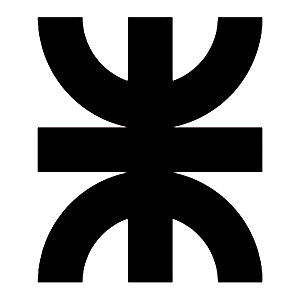
\includegraphics[width=5cm]{utn.png}
		\end{center}
	\end{figure}
	\vspace{5pt}
	\begin{center}
		{\large{FACULTAD REGIONAL PARANÁ}}
		\vspace{5pt}
		\begin{center}
			\vspace{15pt}
			\normalsize{CARRERA: Ingeniería Electrónica\\
						CÁTEDRA: Técnicas Digitales II\\}
			\vspace{50pt}
			\huge\bfseries{Trabajo Práctico N°12\\
			Lectura de iluminación mediante LDR\\}
			\vspace{50pt}
		\end{center}
		
		\begin{flushleft}
			\begin{center}
				ALUMNOS:\\
				Battaglia Carlo\\
				Escobar Gabriel\\
			\end{center}
		\end{flushleft}
		
		\begin{center}
			\vspace{\fill}
			\normalsize{Paraná,}
			\today
		\end{center}
	\end{center}
\end{titlepage}

\newpage
\pagenumbering{arabic}
\numberwithin{equation}{section}

\section{Actividades}

\textbf{1.} El circuito “base” podrá ser el utilizado en el trabajo práctico Nro 8.

\textbf{2.} El circuito deberá tener, además:

\quad \textbf{a.} Un LDR, convenientemente conectado, a una entrada analógica de la placa Arduino.

\textbf{3.} El funcionamiento general del circuito es:

\quad \textbf{a.} El sistema deberá indicar en el display, con un número entre 0 y 9, el grado de “iluminación” presente.

\quad \textbf{b.} Considere los valores adecuados para la comparación, de manera que, para la oscuridad total (LDR tapado) marque 0, y para una fuente de luz que seleccionara acorde, marque 9.

\section{Código}

Al inicio del programa, repetimos las daclaraciones básicas ya conocidas.

Esta vez, inicializamos el ADC mediante la subrutina \textit{init\_ADC} y seleccionamos el canal a utilizar con \textit{Set\_Channel}. Luego inicializamos los puertos a utilizar mediante \textit{init\_port}.

Tal como se indica en el datasheet, descartamos la primera conversión del ADC.

\begin{lstlisting}
Reset:
ldi R16, LOW(RAMEND)
    out SPL, R16
ldi R16, HIGH(RAMEND)
    out SPH, R16

call init_ADC
call init_port
ldi r16,0
rcall Set_Channel
call wait

; Realizo la primera conversión (el resultado es descartado)
rcall Go_Convert
cli
\end{lstlisting}

En el bucle principal, convertimos mediante el ADC el valor presente en el canal seleccionado previamente.

Luego, mediante la función \textit{get\_range} le asignamos un número entre 0 y 9 acorde a su rango.

Finalmente codificamos el valor para poder mostrarlo en el display de 7 segmentos conectado en el puerto D.

\begin{lstlisting}
Loop:
rcall get_ADC
rcall get_range
rcall BCD_to_7_segment
out PORTD, r16
rjmp Loop ; Volver al inicio
\end{lstlisting}

La función \textit{get\_range} asigna un valor entre 0 y 9, dividiendo el valor en cuestión por el ancho de cada rango.

En este caso, dividimos los 1024 valores posibles en rangos de 102. El valor de entrada se divide por este ancho mediante sustracciones sucesivas, hasta obtener como resto el valor correspondiente al rango.

Este método es bastante costoso y resultaría más rápido utilizar una tabla de conversión.

\begin{lstlisting}
get_range:
clr r16
cpi r18, 1
brsh loop_range
cpi r17, 102
brsh loop_range
ret
loop_range:
inc r16
subi r17,low(102)
sbci r18,high(102) ;SE PUEDE PONER 0
cpi r18, 1
brsh loop_range
cpi r17, 102
brsh loop_range
ret
\end{lstlisting}

Rutinas correspondientes al ADC:

\begin{lstlisting}
;===========================================
; Set_Channel
; Selecciona el canal del conversor ADC
; Parámetro: R16 -> canal ha convertir
; Retorno: nada
Set_Channel:
lds r17,ADMUX
andi r17, 0xF0
andi r16, 0x0F
or r16, r17
sts ADMUX, r16
ret
\end{lstlisting}

\begin{lstlisting}
;============================================
; Get_ADC
; Convierte el canal seleccionado previamente
; Parámetro: Nada
; Retorno: R18:R17 -> valor del canal
get_ADC:
{
/* Inicio la conversión */
lds r16, ADCSRA
ori r16, (1<<ADSC)
sts ADCSRA, r16

/* Espero que termine la conversión */
_adc_loop1:
lds r16, ADCSRA
sbrc r16, ADSC
rjmp _adc_loop1
/* Guardo el resultado en R18:R17 */
lds r17, ADCL
lds r18, ADCH
/* Borro la bandera de Interrupción del conversor */                         
lds r16, ADCSRA
sbr r16, (1 << ADIF)
sts ADCSRA, r16

ret
}
\end{lstlisting}

\begin{lstlisting}
;===========================================
; Go_Convert
; Convierte el canal seleccionado
; Parámetro: none
; Retorno: R18:R17 -> valor del canal
Go_Convert:
{
/* Inicio la conversión */
lds r16, ADCSRA
ori r16, (1<<ADSC)
sts ADCSRA, r16

/* Espero que termine la conversión */
_adc_loop:
lds r16, ADCSRA
sbrs r16, ADIF
rjmp _adc_loop
/* Leo y guardo el resultado */
lds r17, ADCL
lds r18, ADCH
/* Borro la bandera de Interrupción del conversor */                         
lds r16, ADCSRA
sbr r16, (1 << ADIF)
sts ADCSRA, r16
ret
}
\end{lstlisting}

\begin{lstlisting}
;===========================================
; init_ADC
; Inicia el ADC
; Habilita ADC, CLK_ADC = 125KHz, V ref = AVCC
; Justificado a derecha, Canal Selec: GND
init_ADC:
; Habilitación del ADC, configuración del prescaler en 128
ldi r16, (1 << ADEN)|(0 << ADATE)|(1 << ADPS2)|(1 << ADPS1)|(1 << ADPS0)
sts ADCSRA, r16

; Referencia del ADC: AVCC, justificado a la derecha y selección del canal GND
ldi r16, (0 << REFS1)|(1 << REFS0)|(0 << ADLAR)|(1 << MUX3)|(1 << MUX2)|(1 << MUX1)|(1 << MUX0)
sts ADMUX, r16
; Configuro "free running mode" pero no se usa el "Auto Trigger"
ldi r16, (0 << ADTS2)|(0 << ADTS1)|(0 << ADTS0)
sts ADCSRB, r16
; Deshabilito la entrada digital para el canal 0
ldi r16, (1 << ADC0D) 
sts DIDR0, r16
ret
\end{lstlisting}

Inicialización de puertos utilizados:

\begin{lstlisting}
;===========================================
; init_port
; Inicia el Puerto PD como salida
init_port:
in r16, DDRD
sbr r16, (1 << DDD7)|(1 << DDD6)|(1 << DDD5)|(1 << DDD4)|(1 << DDD3)|(1 << DDD2)|(1 << DDD1)|(1 << DDD0)
out DDRD, r16
ldi r16, 0
out PORTD, r16
ret
\end{lstlisting}

Conversión de BCD a 7 segmentos mediante tabla de conversión:

\begin{lstlisting}
;===========================================
; BCDTo7Segment
;
; Convierte el valor, pasado en el registro r16, a una representación en 
; display de 7 segmentos, de manera que:
; Dp g f e d c b a
; B7 B6 B5 B4 B3 B2 B1 B0
;
BCD_to_7_segment:
push ZH
push ZL
ldi ZH,HIGH(2*BCDTo7Seg) ; Carga la tabla
ldi ZL,LOW(2*BCDTo7Seg)
add ZL,r16
lpm
mov r16,R0
pop ZL
pop ZH
ret

; Tabla de conversión decimal a 7 segmentos
BCDTo7Seg:
.db 0x3F,0x06,0x5B,0x4F,0x66,0x6D,0x7D,0x07,0x7F,0x6F
\end{lstlisting}

Esta última subrutina fue utilizada para esperar un tiempo determinado y dar lugar a la correcta inicialización del ADC, puesto que la primera conversión siempre tarda más.

\begin{lstlisting}
;
; wait
;
; Demora aprox. 394 mseg
;
wait:
push r16
push r17
push r18

ldi r16,0x20 
ldi r17,0x00 
ldi r18,0x00 
_w0:
dec r18
brne _w0
dec r17
brne _w0
dec r16
brne _w0

pop r18
pop r17
pop r16
ret
\end{lstlisting}

\end{document}
